    
    
    
    

    

    \hypertarget{asyncio---un-exemple-un-peu-plus-ruxe9aliste}{%
\section{\texorpdfstring{\texttt{asyncio} - un exemple un peu plus
réaliste}{asyncio - un exemple un peu plus réaliste}}\label{asyncio---un-exemple-un-peu-plus-ruxe9aliste}}

    \hypertarget{compluxe9ment---niveau-avancuxe9}{%
\subsection{Complément - niveau
avancé}\label{compluxe9ment---niveau-avancuxe9}}

    Pour des raisons techniques, il n'est pas possible de mettre en ligne un
notebook pour les activités liées au réseau, qui sont pourtant
clairement dans le coeur de cible de la bibliothèque - souvenez-vous que
ce paradigme de programmation a été développé au départ par les projets
comme tornado, qui se préoccupe de services Web.

    Aussi, pour illustrer les possibilités offertes par \texttt{asyncio} sur
un exemple un peu plus significatif que ceux qui utilisent
\texttt{asyncio.sleep}, nous allons écrire le début d'une petite
architecture de jeu.

Il s'agit pour nous principalement d'illustrer les capacités de
\texttt{asyncio} en matière de gestion de sous-processus, car c'est
quelque chose que l'on peut déployer dans le contexte des notebooks.

    Nous allons procéder en deux temps. Dans ce premier notebook nous allons
écrire un petit programme Python qui s'appelle \texttt{players.py}.
C'est une brique de base dans notre architecture, dans le second
notebook on écrira un programme qui lance (sous la forme de
sous-processus) plusieurs instances de \texttt{players.py}.

    \hypertarget{le-programme-players.py}{%
\subsubsection{\texorpdfstring{Le programme
\texttt{players.py}}{Le programme players.py}}\label{le-programme-players.py}}

    Mais dans l'immédiat, voyons ce que fait \texttt{players.py}. On veut
modéliser le comportement de plusieurs joueurs.

Chaque joueur a un comportement hyper basique, il émet simplement à des
intervalles aléatoires un événement du type~:

\begin{quote}
je suis le joueur John et je vais dans la direction Nord
\end{quote}

Chaque joueur a un nom, et une fréquence moyenne, et un nombre de
cycles.

Par ailleurs pour être un peu vraisemblable, il y a quatre directions
\texttt{N}, \texttt{S}, \texttt{E} et \texttt{W}, mais que l'on
n'utilisera pas vraiment dans la suite.

    Voyez ici le code de \texttt{players.py}

    Comme vous le voyez, dans ce premier exemple nous n'utilisons à nouveau
que \texttt{asyncio.sleep} pour modéliser chaque joueur, dont la logique
peut être illustrée simplement comme ceci (où la ligne horizontale
représente le temps)~:

    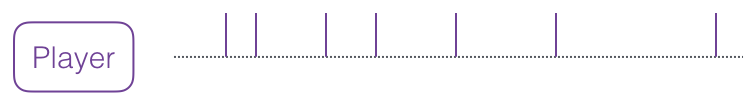
\includegraphics{media/player.png}

    Pour éviter de nous noyer dans des configurations compliquées, on a
embarqué dans \texttt{players} plusieurs configurations prédéfinies,
mais dans tous les cas chacune de ces configurations crée deux joueurs.

    La logique des deux joueurs est simplement juxtaposée, ou si on préfère
superposée, par \texttt{asyncio.gather}, ce qui fait que la sortie de
\texttt{players.py} ressemble à ceci~:

    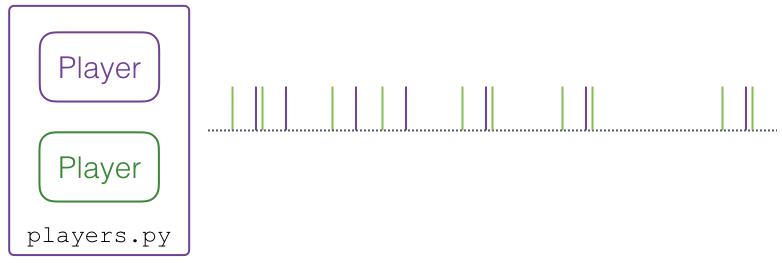
\includegraphics{media/players.png}

    \begin{Verbatim}[commandchars=\\\{\}]
{\color{incolor}In [{\color{incolor}1}]:} \PY{c+c1}{\PYZsh{} je peux lancer un sous\PYZhy{}processus}
        \PY{c+c1}{\PYZsh{} depuis le notebook}
        \PY{o}{!}data/players.py
\end{Verbatim}


    \begin{Verbatim}[commandchars=\\\{\}]
S john
N mary
N mary
E mary
W john
E mary
S mary
E mary
S john
N mary
S john
N mary

    \end{Verbatim}

    \begin{Verbatim}[commandchars=\\\{\}]
{\color{incolor}In [{\color{incolor}2}]:} \PY{c+c1}{\PYZsh{} ou une autre configuration}
        \PY{o}{!}data/players.py \PY{l+m}{2}
\end{Verbatim}


    \begin{Verbatim}[commandchars=\\\{\}]
E bill
W jane
E bill
W jane
S jane
E bill
W jane
S bill
S jane
N bill
E bill

    \end{Verbatim}

    Nous allons voir dans le notebook suivant comment on peut orchestrer
plusieurs instances du programme \texttt{players.py}, et prolonger cette
logique de juxtaposition / mélange des sorties, mais cette fois au
niveau de plusieurs processus.


    % Add a bibliography block to the postdoc
    
    
    
